\documentclass[12pt,letterpaper,fleqn]{article}

\usepackage[utf8]{inputenc}
\usepackage{tikz}
\usepackage[utf8]{inputenc}
\usepackage[T1]{fontenc}
\usepackage{amsmath}
\usepackage{amssymb}
\usepackage{multicol}
\usepackage{graphicx}
\usepackage{mdwlist}
\usepackage{ upgreek }
\usepackage{ stmaryrd }


\usepackage[dvipsnames]{xcolor}
\usepackage[most]{tcolorbox} 

\usepackage{tabu}

\usepackage{mathtools}

\usepackage[top=1in, bottom=1in, left=1in, right=1in]{geometry}


\begin{document}

    \begin{titlepage}
        \centering
        {\scshape\LARGE Universidad Nacional Autónoma de México \par}
    
        \vspace{0.5cm}
        {\scshape\LARGE Facultad de Ciencias\par}
    
        \begin{center}
            \includegraphics[scale=.6]{logo.png}
        \end{center}
    
        {\scshape\LARGE \textbf{Tarea 04}\par}
        
       \vspace{.5 cm}
    
        {\scshape Presentan\par}
        \begin{center}
            \begin{itemize}
                \centering
                \item Nelson Osmar Garcia Villa - 322190357
                \item Valeria Camacho Hernández - 322007273
                \item Mauricio Casillas Álvarez - 322196342
            \end{itemize}
        \end{center}
        
        \vspace{.5 cm}

        {\scshape Asignatura \par}
        \begin{center}
            Gráficas y Juegos 2025-2
        \end{center}

            
        \vspace{.5 cm}

        {\scshape Profesor \par}

        \begin{center}
            César Hernández Cruz
        \end{center}

        \vspace{.5 cm}
        
        {\scshape Ayudante \par}
        
        \begin{center}
        Iñaki Cornejo de la Mora
        \end{center}
        
        \vspace{.5 cm}

        {\scshape Fecha \par}
        \begin{center}
        Viernes 07 de marzo del 2025
        \end{center}
        
        \vfill
    \end{titlepage}
    
\begin{center}
    \LARGE{\textbf{Tarea 04}}
\end{center}

\begin{enumerate}
  \item Sea $G$ una gr\'afica no trivial.   Demuestre que $G$ es una trayectoria
    si y s\'olo si $G$ es un \'arbol con exactamente dos v\'ertices de grado
    $1$.
    
    \underline{Respuesta:} 

    $\Rightarrow)$ Tenemos que una trayectoria es una gráfica conexa que no contiene ciclos y en la que todos los vértices tienen grado 2, excepto dos vértices (los extremos) que tienen grado 1. Como una trayectoria es conexa y no tiene ciclos, es un árbol. Además, los dos vértices extremos de la trayectoria tienen grado 1, y todos los demás vértices tienen grado 2.

    $\therefore$ $G$ es un árbol con exactamente dos vértices de grado 1.

   $\Leftarrow$ Una gráfica \( G \) es conexa y no tiene ciclos, lo que lo hace un árbol, además, si $G$ es un árbol, tiene exactamente dos vértices de grado 1, siendo ambos vértices, son las hojas del árbol.
   
   Ahora, un árbol con exactamente dos vértices de grado 1 debe ser una estructura lineal. Si hubiera más de dos vértices de grado 1, el árbol tendría ramificaciones, lo que contradice la hipótesis.
   
   Dado que \( G \) es conexo y no tiene ciclos, existe un único camino entre los dos vértices de grado 1. Este camino incluye todos los vértices del árbol, ya que si hubiera vértices fuera de este camino, \( G \) no sería conexo o tendría más de dos vértices de grado 1.

    $\therefore$ $G$ es una trayectoria, ya que es un camino que conecta los dos vértices de grado 1 sin ciclos.

    Por lo tanto, $G$ es trayectoria si y sólo si $G$ es un árbol con exactamente dos vértices de grado $1$. $\bigstar$

\begin{enumerate}
    \item Demuestre que cada \'arbol con grado m\'aximo $\Delta > 1$ tiene al
      menos $\Delta$ hojas. 

       \underline{Respuesta:}

       Sea $T$ un árbol $n$ vértices y un vértice $v$ tal que su grado es $\Delta$, es decir el vértice con más aristas del arbol, mayor a 1.

       Supongamos por contradicción que el árbol tiene menos de $\Delta$ hojas.

       Si $v$ tiene $\Delta$ aristas y el árbol tiene menos de $\Delta$ hojas entonces existe algún vecino en $v$ que tiene grado mayor que 1, como hay hojas $<$ a $\Delta$ implica que el vecino no sea una hoja, por lo que hay otra arista conectada entre sí o a otros vértices. 

       Considerando el vértice $v$ como grado mayor a 1, como $u$ no es hoja (ya que una hoja solo tiene un grado máximo), tiene al menos un vecino $u$, entonces este vecino tampoco es hoja, buscando nuevamente un vértice vecino que sea hoja. Pero $T$ es un árbol si continuamos con este proceso, eventualmente llegaremos a un vértice de grado 1. Llegando a una contradicción, ya que un árbol es finito y cada vértice está conectado de forma aciclica, no podemos avanzar de fomra indefinida sin encontrar una hoja que enseñe hasata donde llega el camino en la estructura. 

      $\therefore$ Cada árbol con grado máximo $\Delta > 1$ tiene el menos $\Delta$ hojas.

       \newpage
       
  	\item Construya, para cada elecci\'on de $n$ y $\Delta$, con $2\le \Delta <
      n$, un \'arbol de orden $n$ con exactamente $\Delta$ hojas.
  	\end{enumerate}
        
        \underline{Respuesta:}
        
         \hfill Para $\Delta$=1 ; $n=2$ 
                
            \begin{center}
                
                \begin{tikzpicture}[scale=3]
                \coordinate (A) at (0.2,0.0,0.8);
                \coordinate (B) at (0.76,0.4,0.2);

                \draw[thick] (A) -- (B);
                                
                \node [draw, circle] at (A) [below left] {$A$};
                \node [draw, circle] at (B) [above right] {$B$};
                              
                \end{tikzpicture}

            \end{center}
    
        \hfill Para $\Delta$=2 ; $n=3$ 
                
            \begin{center}
                
                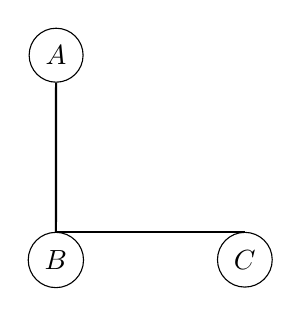
\begin{tikzpicture}[scale=3]
                \coordinate (A) at (-0.03,0.4,0.2);
                \coordinate (B) at (0.2,0.0,0.8);
                \coordinate (C) at (1,0.0,0.8);

                \draw[thick] (A) -- (B);
                \draw[thick] (B) -- (C);
                                
                \node [draw, circle] at (A) [above] {$A$};
                \node [draw, circle] at (B) [below] {$B$};
                \node [draw, circle] at (C) [below] {$C$};
               
                \end{tikzpicture}

            \end{center}

            \hfill Para $\Delta$=2 ; $n=4$ 
                
            \begin{center}
                
                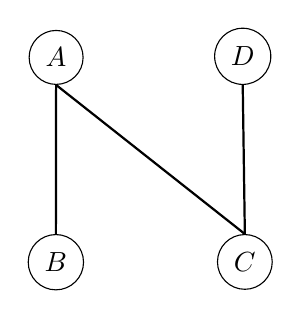
\begin{tikzpicture}[scale=3]
                \coordinate (A) at (-0.03,0.4,0.2);
                \coordinate (B) at (0.2,0.0,0.8);
                \coordinate (C) at (1,0.0,0.8);
                \coordinate (D) at (0.76,0.4,0.2);

                \draw[thick] (A) -- (B);
                \draw[thick] (A) -- (C);
                \draw[thick] (C) -- (D);
                                
                \node [draw, circle] at (A) [above] {$A$};
                \node [draw, circle] at (B) [below] {$B$};
                \node [draw, circle] at (C) [below] {$C$};
                \node [draw, circle] at (D) [above] {$D$};
               
                \end{tikzpicture}

            \end{center}
            
            
       

  \item Un {\em centro} en una gr\'afica es un v\'ertice $u$ tal que $\max_{v
    \in V} d(u, v)$ es m\'inima. Demuestre que un \'arbol tiene exactamente un
    centro o dos centros adyacentes.

    \underline{Respuesta:} Sea $T$ un árbol.

    Casos Base:
    \begin{itemize}
        \item Si $T$ tiene $n=1$ vértice, ese es el centro (por definición de centro), pues no hay otros vértices por lo que su $excentricidad =0$.
        \item Si $T$ tiene $n=2$ vértices, ambos son el centro (por definición de centro), pues ya están conectados y tiene la misma $excentricidad=1$, la cual es la mínima posible.
    \end{itemize}

    Paso Inductivo: Supongamos que para cualquier árbol $T$ con $k$ vértices, tales que $k \geq 2$, su centro es uno o son dos adyacentes.

    Por demostrar: Sea $T$ un árbol con $n=k+1$ vértices.

    Procedemos eliminando cada una de todas las hojas (vértices de grado 1) de $T$ hasta llegar a su centro. Al eliminar las hojas de un árbol $T$, obtenemos un nuevo árbol $T'$, que conserva los mismo centros que $T$, es decir, $T'$ es un subárbol de $T$. Las hojas no pueden ser centros porque tienen $excentricidad$ máxima, pues están en los extremos del árbol. Al eliminar las hojas, las distancias entre los vértices restantes no aumenta, ya que las hojas no están no pueden ser el centro, o centros, del árbol. Además, las trayectorias más largas (diámetros) se acortan, pero donde se encuentra el centro no cambia. 
    
    Además, consideremos que en un árbol, la trayectoria más larga (diámetro) es el camino más extenso entre dos hojas. Si el diámetro tiene una longitud par, hay un único vértice en el "medio" de esta trayectoria, que es el centro. Si el diámetro tiene una longitud impar, hay dos vértices en el "medio" de esta trayectoria, que son los dos centros adyacentes. Entonces, esta trayectoria no se ve afectada por la eliminación de hojas, pues estas están en los extremos del árbol, lo que no altera las distancias entre los vértices restantes.

    En cada eliminación, el número de vértices se hace menos. Cuando ya no encontramos más hojas que eliminar, es porque tenemos uno o dos vértices. Entonces, los vértices que quedan en $T'$ mantienen sus distancias relativas . Si $T'$ tiene un solo vértice, ese centro es el único, mientras que si tiene dos vértices adyacentes, ambos son centros (adyacentes).

    
    Como las hojas no pueden ser centros, pues tienen excentricidad máxima, el centro de $T$ es el mismo que de $T'$, por lo que este proceso de ir eliminando hojas nos lleva a encontrar el centro, o centros, del árbol $T$.

    $\therefore$ $T$ tiene un centro o dos centros adyacentes.

    Por lo tanto, todo árbol tiene un centro o dos centros adyacentes. $\bigstar$

  \item Demuestre o brinde un contraejemplo: Toda gr\'afica con menos aristas
    que v\'ertices tiene una componente que es un \'arbol.
    
    \underline{Respuesta:}  Una gráfica con \( n \) vértices y \( m \) aristas, donde \( m < n \), debe tener al menos una componente conexa que es un árbol.  

    Si una gráfica tiene menos aristas que vértices (\( m < n \)), entonces no puede ser conexa, ya que una gráfica conexa con \( n \) vértices tiene al menos \( n-1 \) aristas.  

    Por lo tanto, debe tener al menos una componente conexa que es un árbol, ya que, por definición, si todas las componentes fueran cíclicas, tendría al menos \( n \) aristas, lo que contradice \( m < n \).   $\blacksquare$
    

  \item Un \textit{hidrocarburo saturado} es una mol\'ecula $C_mH_n$ en la que
    cada \'atomo de carbono tiene cuatro enlaces, cada \'atomo de hidr\'ogeno
    tiene un enlace, y ninguna sucesi\'on de enlaces forma un ciclo. Demuestre
    que para cualquier entero positivo $m$, la mol\'ecula $C_mH_n$ existe s\'olo
    si $n = 2m + 2$.

    \underline{Respuesta:} 

    \begin{enumerate}
        \item Cada átomo de carbono se representa como un vértice en el árbol.
        \item Cada átomo de hidrógeno se representa como una hoja en el árbol.
        \item Cada enlace se representa como una arista en el árbol.
        \item Los átomos de hidrógeno están conectados a átomos de carbono, que si grado sea menor a 4.
    \end{enumerate}

    Como cada átomo de carbono tiene cuatro enlaces (no especifica a que átomo está conectado) y hay $m$ átomos de carbono, entonces podemos denotar el grado de los átomos de carbono como $4m$. Pero si existe un enlace de átomo de carbono conectado a otro átomo de carbono, y como una arista se cuenta dos veces, una para cada vértice de carbono que conecta, el número de aristas totales queda como: $\frac{4m}{2}=2m$.
    
    Ahora aquel vértice de grado uno, es decir algún vértice que no está conectado a otro vértice, se tiene un átomo de hidrógeno al inicio y al final de las cadenas de hidrocarburo saturado, implica que existe la ausencia de 2 átomos de hidrógenos para completar los cuatro enlaces, entonces el número de total de átomos de hidrógeno $n$ es igual al número de aristas totales más 2 $\Rightarrow$ $n=2m+2$.
    
    $\therefore$ La mol\'ecula $C_mH_n$ existe s\'olo si $n = 2m + 2$. 

  \item Demuestre que una sucesi\'on $(d_1, \dots, d_n)$ de enteros positivos es
    la sucesi\'on de grados de un \'arbol si y s\'olo si $\sum_{i=1}^n d_i =
    2(n-1)$.

    \underline{Respuesta:} Construimos ambos lados.
    
    $(\Rightarrow)$: Si $(d_{1}, d_{2}, ..., d_{n})$ es la sucesión de grados de un árbol, entonces, la suma de los grados debe de ser $\sum_{i=1}^n d_i$. Como un árbol con $n$ vértices tiene $n-1$ aristas, y cada arista tiene dos extremos, es decir, a la suma de los grados de los vértices le añadimos dos unidades, la suma de los grados de los vértices es dos veces el número de aristas. Por lo tanto, la suma de los grados $2(n-1)$.

    $\therefore$ La sucesión de grados corresponde a un árbol cumpliendo \(2(n-1) = \sum_{i=1}^n d_i\).

    $(\Leftarrow)$: Si la suma de los grados es $2(n-1)$, entonces la gráfica es un árbol, es decir, es conexa y no tiene ciclos.

    Primero veamos que la sucesión de grados corresponda a una gráfica. Para ello, la suma de todos los grados en la sucesión debe ser par. Esto se debe a que cada arista contribuye con $2$ a la suma total de grados (uno para cada vértice que conecta). Si la suma es impar, la sucesión no puede corresponder a una gráfica. Sabemos que en cualquier gráfica, la suma de los grados de todos los vértices es igual a dos veces el número de aristas, $2m$ con $m$ como el número de aristas. En un árbol, $m=n-1$. Veamos más detalladamente esto.

    Caso base:
    Sea $n=1$. Este es un árbol con un solo vértice sin aristas, $m=0$, entonces la suma de grados es $0$, es decir $2(n-1)=0$. Esto cumple ser conexo y sin ciclos (un árbol).

    Paso inductivo: Supongamos que para para cualquier árbol con $k$ vértices, si la suma de grados es $2(k-1)$, entonces corresponde a una gráfica que es un árbol (conexa y sin ciclos).

    Por demostrar: Sea $T$ una gráfica con $k+1$ vértices y la suma de grados $2(k)$, entonces $T$ es un árbol.

    En cualquier gráfica con $k+1$ vértices y la suma de grados $2(k)$, debe existir al menos un vértice de grado 1 (es una hoja). Esto se debe a que si todos los vértices tuvieran grado mayor o igual a $2$, la suma de grados sería al menos $2(k+1)$, lo cual contradice $\sum d_i =2(k)$. 
    
    Al eliminar una hoja $v$ junto con la arista que la conecta al resto de la gráfica, resulta en una nueva gráfica $T'$ con $k$ vértices, con la suma de grados siguiente:

    \(\sum_{i=1}^k d'_i = 2(k) - 2 =2(k-1)\).

    Esta resulta en la hipótesis inductiva. Luego, por hipótesis, $T'$ es un árbol (conexo y sin ciclos) con $k$ vértices Y $k-1$ aristas.

    Ahora al agregar de nuevo la hoja $v$ y su arista a $T$, obtenemos $T$, quien tiene $k+1$ vértices y $k$ aristas. Además, como $T'$ es conexo y sin ciclos, $T$ también es coenxo y sin ciclos, pues agregar una hoja no introduce ciclos (porque una hoja tiene grado $1$ y no puede formar parte de un ciclo) ni desconexiones (porque la hoja está conectada directamente a un vértice del árbol original, manteniendo la conexidad).

    Así, cualquier gráfica con $n$ vértices y la suma de grados $2(n-1)$ es un árbol (conexo y sin ciclos).
    
    $\therefore$ \(\sum_{i=1}^n d_i = 2(n-1)\).

    Por lo tanto, \(\sum_{i=1}^n d_i = 2(n-1)\). $\bigstar$
    
\end{enumerate}

\section*{Puntos Extra}
\begin{enumerate}

  \item Para una gr\'afica conexa $G$ definimos la gr\'afica de \'arboles de
    $G$, $\mathcal{T}_G$, como la gr\'afica que tiene por v\'ertices a todos los
    \'arboles generadores de $G$, y tal que, si $S, T \in V_{\mathcal{T}_G}$,
    entonces $ST$ es una arista de $\mathcal{T}_G$ si y s\'olo si existen
    aristas $e \in E_S - E_T$ y $f \in E_T - E_S$ tales que $(S - e) + f = T$.
    Demuestre que $\mathcal{T}_G$ es conexa.

    \underline{Respuesta:} 
    
    Caso Base: Si \( S = T \), entonces trivialmente están conectados.

    Paso inductivo: Supongamos que \( S \) y \( T \) son dos árboles generadores distintos de \( G \). Queremos mostrar que existe una secuencia de árboles generadores \( S = T_0, T_1, \ldots, T_n = T \) tal que cada par consecutivo \( T_i \) y \( T_{i+1} \) está conectado por una arista en \( T_G \).

    Construcción del camino: Dado que \( S \) y \( T \) son árboles generadores, tienen el mismo número de aristas.
    
    Consideremos la diferencia simétrica de las aristas de \( S \) y \( T \), es decir, \( E_S \triangle E_T \).
    
    En cada paso, seleccionamos una arista \( e \) en \( E_S - E_T \) y una arista \( f \) en \( E_T - E_S \) tal que al reemplazar \( e \) por \( f \) en \( S \), obtenemos un nuevo árbol generador \( S' \). Este proceso se repite hasta que \( S' = T \). Cada paso corresponde a una arista en \( T_G \), lo que garantiza que existe un camino entre \( S \) y \( T \).
 
    Hemos mostrado que para cualquier par de árboles generadores \( S \) y \( T \) en \( T_G \), existe un camino en \( T_G \) que los conecta. Por lo tanto, \( T_G \) es conexa. $\blacksquare$
    

  \item Sea $T$ un \'arbol arbitrario con $k+1$ v\'ertices. Demuestre que si $G$
    es simple y $\delta \ge k$, entonces $G$ tiene una subgr\'afica isomorfa a
    $T$.

    \underline{Respuesta:} Sea $T$ un árbol arbitrario con $k+1$ y sea $G$ una gráfica simple (sin lazos ni aristas múltiples) con $\delta \ge k$. Es decir, $T$ es un árbol, que conecta $k+1$ vértices sin formar ciclos (por definición de árbol), y $G$ es una gráfica sin lazos ni conexiones repetidas que tiene grado mímino $\delta$, por lo que cada punto de $G$ está conectado al menos con $k$ otros puntos.

    Por demostrar: Dentro de $G$ podemos encontrar una parte, osea una subgráfica, que sea exactamente igual a $T$, es decir, con la misma estructura de conexiones entre los vértices. Procedemos por construcción.

    Como $G$ tiene al menos $k+1$ vértices, ya que cada vértice en $G$ tiene al menos $k$ vecinos, entonces hay suficientes vértices para formar $T$, por lo que seleccionamos un vértice cualquiera $v$ en $G$ y lo asignamos a la raíz de $T$.

    El árbol $T$ tiene una su raíz con hijos. Supongamos que la raíz de $T$ tiene $d$ hijos, con $d \leq k$. Como $G$ tiene grado mínimo, $\delta(G) \geq k$, el vértice $v$ en $G$ tiene al menos $k$ vecinos. Si tomamos $d$ de eso vecinos y los asignamos como hijos a la raíz de $T$, una parte de $T$ ya está dentro de $G$, respetando las conexiones.

    Ahora, seguimos expandiendo $T$ de la misma manera detallada previamente: Tomamos un vértice $u$ que ya asignamos en $G$, es decir, un vértice que ya tiene su copia en $G$, y observamos sus hijos en $T$ para asignarlos a los vecinos no usados de $u$ en $G$. Este proceso se repite para cada nuevo vértice agregado hasta que todos los vértices de $T$ están asignados en $G$.
    
    $\therefore$ Como siempre hay suficientes vértices y siempre podemos respetar las conexiones, se cosntruyó una subgráfica $G$ isomorfa a $T$. 

    Por lo tanto, $G$ tiene una subgráfica isomorfa a $T$. $\bigstar$


  \item Sea $\mathcal{T}$ una familia de sub\'arboles de un \'arbol $T$.
    Demuestre que si cualesquiera dos elementos de $\mathcal{T}$ tienen un
    v\'ertice en com\'un, entonces hay un v\'ertice de $T$ que est\'a en todos
    los elementos de $\mathcal{T}$.

    \underline{Respuesta:} 
    
    Supongamos que no existe un vértice común a todos los subárboles de \( \mathcal{T} \).  
    Entonces, para cada vértice \( v \) en \( T \), existe al menos un subárbol en \( \mathcal{T} \) que no contiene \( v \).  

    Como \( T \) es un árbol, es conexo y no tiene ciclos. Por lo tanto, si dos subárboles comparten un vértice y cualquier par de subárboles comparte al menos un vértice, debe existir un vértice común a todos los subárboles.  
    
    Esto se debe a la propiedad de intersección finita de los árboles: si cualquier par de subárboles tiene intersección no vacía, entonces la intersección de todos los subárboles también es no vacía.  

    Por lo tanto, existe un vértice \( T \) que está en todos los subárboles de \( \mathcal{T} \).  $\blacksquare$

  \item \begin{enumerate}
    \item Determine todos los arboles $T$ tales que $\overline T$ tambi\'en es
      un \'arbol.
      
      \underline{Respuesta:} 

      Sabemos que $T$ es un árbol con $n$ vértices y como lo vimos en clase con $n-1$ aristas

      Si el número total de aristas que tiene una gráfica de $n$ vértices es ${n \choose 2}=\frac{n(n-1)}{n}$, pero como sabemos un árbol no puede ser completo, porque rompe con su característica de no tener ciclos, entonces si $\overline T$ es un árbol y tiene aquellas aristas que no aparecen en $T$, podemos saber que las aristas de $\overline T={n \choose 2}-n-1$ se obtienen al restar las aristas que hay en un árbol $T$ con el número total de aristas que hay en una gráfica es decir:
      
      \begin{center}
          Número de aristas de $\overline T=\frac{n(n-1)}{2}-(n-1)$
      \end{center} 

      Pero si $\overline T$ también es un árbol entonces sabemos que el número de aristas de un árbol es $n-1$ sustituimos:

      \begin{center}
          $n-1 =\frac{n(n-1)}{2}-(n-1)$
      \end{center} 
      Resolvemos la ecuación
      
      Sacamos el 2 dividiendo, multiplicando toda la ecuación por dos 
      \begin{center}
          $\Rightarrow 2(n-1)=n(n-1)-2(n-1)$ 
      \end{center} 
      Pasamos lo que está restando al otro lado sumando

      \begin{center}
          $\Rightarrow 2(n-1)+2(n-1)=n(n-1)$ 
      \end{center}     

      Sumamos

      \begin{center}
          $\Rightarrow 4(n-1)=n(n-1)$ 
      \end{center} 

      Dividimos el lo que esta multiplicando al otro lado dividiendo

      \begin{center}
          $\Rightarrow n=4(\frac{n-1}{n-1})$ 
      \end{center} 

      Quedando 

      \begin{center}
          $\Rightarrow n=4$ 
      \end{center} 

      Entonces el árbol $T$ cuando tiene $n$ vértices igual a $4$, $\overline T$ también es un árbol con $n$ igual a $4$ vértices pero con las aristas que no tiene el árbol $T$.


    \item Determine todas las gr\'aficas de orden al menos cuatro tales que la
      subgr\'afica inducida por cualesquiera tres de sus v\'ertices es un
      \'arbol.
      
      \underline{Respuesta:} 
      
      Tenemos una gráfica $G$ de orden al menos cuatro, y la gráfica inducida de tres vértices es aquella gráfica que se obtiene al tomar tres vértices y las aristas que existían en $G$ entre esos.
      Si cualesquiera tres vértices es un árbol, quiere decir que la gráfica inducida debe de ser aciclica y debe de ser conexa. 
      
      Si tenemos una gráfica $G$ que es un $C_4$ se ve de la siguiebte manera:

      \begin{center}
                
                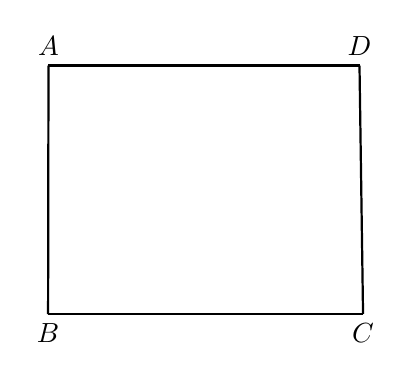
\begin{tikzpicture}[scale=5]
                \coordinate (A) at (-0.03,0.4,0.2);
                \coordinate (B) at (0.2,0.0,0.8);
                \coordinate (C) at (1,0.0,0.8);
                \coordinate (D) at (0.76,0.4,0.2);

                \draw[thick] (A) -- (B);
                \draw[thick] (A) -- (D);
                \draw[thick] (C) -- (D);
                \draw[thick] (B) -- (C);
                                
                \node  at (A) [above] {$A$};
                \node  at (B) [below] {$B$};
                \node  at (C) [below] {$C$};
                \node  at (D) [above] {$D$};
               
                \end{tikzpicture}

            \end{center}
      Está gráfica para todos los casos en que sea una subgráfica inducida de cualesquiera 3 vértices es un árbol cumple la condición.

      \begin{enumerate}
      \item Como se observó en el inciso anterior, demostramos que si $T$ es un árbol y $\overline T$ también es un árbol, entonces $T$ debe tener exactamente 4 vértices.
      
      \item Sabemos que un árbol $T$ con 4 vértices tiene 3 aristas. Si agregamos las aristas faltantes, es decir las aristas que no hay en $T$ pero que si están en $\overline{T}$, nos forma un $C_4$ de manera que siga cumpliéndose la propiedad de que cualquier subgráfica inducido por 3 vértices sea un árbol.
      \end{enumerate}

      No existen otras gráficas de orden 4 que cumplan la propiedad, porque cualquier otra aristas generaría un ciclo de tres vértices ($K_3$) en alguna subgráfica inducida.
      
      $\therefore$ La única gráfica que cumple con la característica de ser gráfica de orden al menos cuatro, tal que su gráfica inducida por cualesquiera tres vértices es un árbol, es la gráfica $C_4$.
      
    \end{enumerate}

     
     

\end{enumerate}

\end{document}

